\section{Introduction} 
An induction coupler uses magnetic eddy currents to create forces between itself and the conductive materials that make up a target. The coupler requires no mechanical contact with a target, nor does it demand cooperation from the target. The coupler can also operate on electricity alone, rather than requiring propellant. Because most satellites include conductive material in their structure—notably aluminum honeycomb with aluminum facesheets or aluminum beams—induction couplers may be the closest thing we have to science fiction's tractor beam: a device that can produce  contactless forces on an uncooperative target. 
Induction couplers show promise for spaceflight applications, offering three major advantages. First, the small forces associated with magnetic fields across meter-scale distances can dominate gravity, friction, aerodynamic drag, and other effects, which are far less pronounced in orbit than in a terrestrial environment. Second, fully deployed spacecraft rarely offer straightforward means for mechanical grappling; so, the ability to interact without the potential for contact damage is valuable. Third, induction couplers offer the ability to maneuver without expendables, eliminating risks associated with propellant-plume impingement and extending the useable lifetime of a spacecraft.
A small spacecraft could use an induction coupler to control its motion relative to a much larger target like the International Space Station (ISS), crawling along the target’s surface without ever touching. This on-orbit inspection technique resembles the locomotion and functions of underwater robots that now inspect pipelines and shipwrecks. 
 
Current interest in on-orbit servicing (OOS) is a strong motivation for advancing induction coupler technology. One of the fundamental technological use cases is that of a small inspection vehicle whose interactions with the target do not produce significant motion in that target—for example, an ISS inspection vehicle. Such a vehicle is primarily concerned with regulating planar motion along the surface of the target and stabilization of out-of-plane translation. This paper  describes a study of how the planar component of that motion can be achieved with induction couplers. 
<<<<<<< HEAD
\begin{figure}
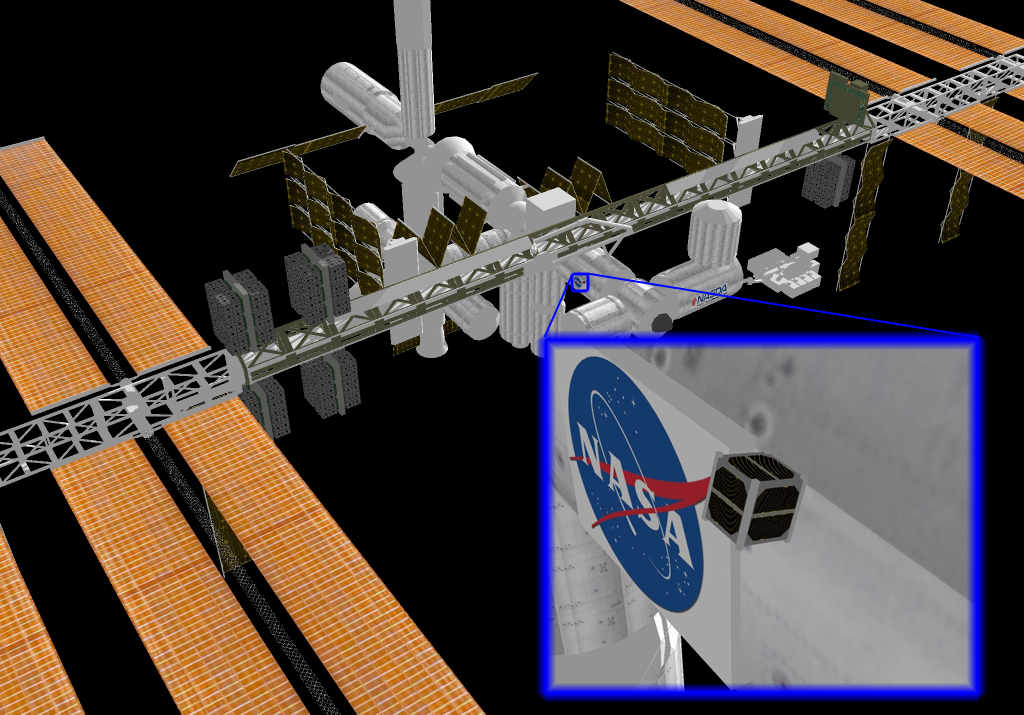
\includegraphics[scale=0.25]{figures/iss_inspector.jpg}
\label{fig:iss_inspector}
\end{figure}
=======

\ref{fig:iss}
>>>>>>> 71718f046e2f513e0b67666fc62b88c2bfa804b5

